% !TeX spellcheck = de_DE
\documentclass[12pt]{article}
\usepackage[utf8]{inputenc}
\usepackage{geometry}
\usepackage{svg}
\usepackage{float}
\usepackage{caption}
\usepackage{amsmath,amsthm,amsfonts,amssymb,amscd}
\usepackage{fancyhdr}
\usepackage{titlesec}
\usepackage{hyperref}
\usepackage{listings}
\usepackage[skip=3pt]{parskip}
\usepackage[ngerman]{babel}
\pagestyle{empty}
\titleformat*{\section}{\large\bfseries}
\titleformat*{\subsection}{\bfseries}

%
\geometry{
	a4paper,
	total={170mm,240mm},
	left=20mm,
	top=30mm,
}

\date{}
%Bitte ausfüllen
\newcommand\course{Betriebssysteme}
\newcommand\hwnumber{\large Portfolio 2}
\newcommand\Name{Fabian Sponholz}
\newcommand\Neptun{1561546}

%Matheinheiten
\newcommand\m{\:\textrm{m}}
\newcommand\M{\:\Big[\textrm{m}\Big]}
\newcommand\mm{\:\textrm{mm}}
\newcommand\MM{\:\Big[\textrm{mm}\Big]}
\newcommand\un{\underline}
\newcommand\s{\:\textrm{s}}
\newcommand\bS{\:\Big[\textrm{S}\Big]}
\newcommand\ms{\:\frac{\textrm{m}}{\textrm{s}}}
\newcommand\MS{\:\Big[\frac{\textrm{m}}{\textrm{s}}\Big]}
\newcommand\mss{\:\frac{\textrm{m}}{\textrm{s}^2}}
\newcommand\MSS{\:\Big[\frac{\textrm{m}}{\textrm{s}^2}\Big]}

%Trennlinie
\newcommand\separator{\rule{\linewidth}{0.5pt}}

%Bitte nicht einstellen
\renewcommand{\figurename}{Abbildung}
\renewcommand{\tablename}{Tabelle}
\pagestyle{fancyplain}
\headheight 35pt
\lhead{\Name\\\Neptun}
\chead{\textbf{ \hwnumber}}
\rhead{\course \\ \today}
\lfoot{}
\cfoot{}
\rfoot{\small\thepage}
\headsep 1.5em

\lstset{
	basicstyle=\ttfamily\small,
	columns=fullflexible,
	frame=single,
	frameround=tttt,
	rulecolor=\color{gray},
}
% http://www.bollchen.de/blog/2011/04/good-looking-line-breaks-with-the-listings-package/
\lstset{
	prebreak=\raisebox{0ex}[0ex][0ex]{\ensuremath{\hookleftarrow}},
	postbreak=\raisebox{0ex}[0ex][0ex]{\ensuremath{\hookrightarrow\space}},
	breaklines=true,
	breakatwhitespace=true,
	numbers=left,
	numberstyle=\scriptsize,
}
\lstset{
	backgroundcolor=\color{white},
	extendedchars=true,
	basicstyle=\footnotesize\ttfamily,
	showstringspaces=false,
	showspaces=false,
	numbers=left,
	numberstyle=\footnotesize,
	numbersep=9pt,
	tabsize=2,
	breaklines=true,
	showtabs=false,
	captionpos=b
}
\lstset{
	keywordstyle=\color{blue}\bfseries,
	ndkeywordstyle=\color{darkgray}\bfseries,
	identifierstyle=\color{black},
	commentstyle=\color{purple}\ttfamily,
	stringstyle=\color{red}\ttfamily
}

\begin{document}
	
\section*{Umgebung der Experimente}
Folgende Tabellen beschreiben das System, auf dem die Tests durchgeführt wurden.
\subsection*{Hardware-Spezifikation}
\begin{table}[h]
	\centering
	\begin{tabular}{|l|l|}
		\hline
		\textbf{Merkmal} & \textbf{Spezifikation} \\
		\hline
		CPU-Bezeichnung & AMD Ryzen 5 4500U with Radeon Graphics\\
		CPU-Architektur & x86 (AMD Renoir) \\
		CPU-Fertigungsverfahren & 7 nm (TSMC) \\
		\hline
		Anzahl Kerne / Threads & 6 / 6 \\
		Basistaktfrequenz & 2.3 GHz \\
		Maximale Boost-Taktfrequenz & 4.0 GHz \\
		\hline
		L1-Cache & 384 KB \\
		L2-Cache & 3 MB \\
		L3-Cache & 8 MB \\
		\hline
		TDP (Thermal Design Power) & 15 Watt \\
		Maximale Temperatur & 105 °C \\
		\hline
		Arbeitsspeicher & 2x4GB DDR4-3200 (Dual Channel) \\
		\hline
		Erscheinungsdatum & 07.01.2020 \\
		\hline
	\end{tabular}
\end{table}

\subsection*{Software-Umgebung}
\begin{table}[h]
	\centering
	\begin{tabular}{|l|l|}
		\hline
		\textbf{Merkmal} & \textbf{Spezifikation} \\
		\hline
		Betriebssystem & Arch Linux\\
		Kernel-Version & Linux 6.12.8-arch1-1\\
		\hline
		Java-Version & Java 21\\
		Java-Implementierung & java-21-openjdk\\
		\hline
		ZeroMQ-Implementierung & JeroMQ 0.6.0\\
		\hline
	\end{tabular}
\end{table}

\section{Aufgabe 1 - Latenz bei Kommunikation mit Spinlock}
\subsection{Erste Ansätze zur Latenzmessung}
Bei der Kommunikation über Spinlocks wartet ein Thread auf die Freigabe einer Ressource, indem er fortwährend (z.B. in einer \texttt{while}-Schleife) überprüft, ob die Ressource frei ist. 
Um die Latenz zu messen, habe ich neben dem Main-Thread einen \texttt{Reader}-Thread erstellt, der auf die Freigabe einer Ressource (Boolean, der auf \texttt{true} gesetzt wird) wartet, und den Wert dann wieder auf \texttt{false} setzt. 
Nachdem der Main-Thread den Wert auf \texttt{true} gesetzt hat, wartet er wiederum, bis der Wert wieder auf \texttt{false} gesetzt wird.

Um Race Conditions beim Abfragen der Werte aus den While-Schleifen zu vermeiden, wird der Zugriff mithilfe von \texttt{synchronized} Setter- und Getter-Methoden geregelt.
Jeder Thread trägt immer, wenn er eine Nachricht vom anderen Thread erhält, einen Zeitstempel in Nanosekunden in eine ausreichend große Array-Liste ein, woraus später die Latenz berechnet wird.
Nun folgen Auszüge aus dem Source Code, die dies zeigen.

\begin{lstlisting}[language=java,caption={Spinlocks: Latenzmessung im Main Thread}]
for (int i = 0; i < recursions; i++) {
	// set lock to true -> send message
	setLock(true);;
	
	// wait for the return message
	while (getLock()) {
		// Do nothing (spinlock)
	}
	
	// add current time to list
	messageTimes.add(System.nanoTime());
}
\end{lstlisting}

\begin{lstlisting}[language=java,caption={Spinlocks: Latenzmessung im Reader Thread}]
while (!isInterrupted()) {
	while (!isInterrupted() && experiment.getLock() == false) {
		// do nothing (spinlock)
	}
	
	// Add the current time to the list
	experiment.getMessageTimes().add(System.nanoTime());
	
	if (isInterrupted()) break;
	
	// Reset the lock (main thread is waiting)
	experiment.setLock(false);
}
\end{lstlisting}


\subsection{Versuchsaufbau / Implementierung}
Im Ursprünglichen Versuchsaufbau habe ich für jeden Versuchsdurchlauf den \texttt{Reader}-Thread und das \texttt{Experiment}-Objekt neu erstellt und jeweils von jedem Experiment die minimale Latenz gespeichert.
Das Ergebnis des ersten Durchlaufs ist in Abbildung \ref{img:spinlock_first} dargestellt.

\begin{figure}[H]
	\centering
	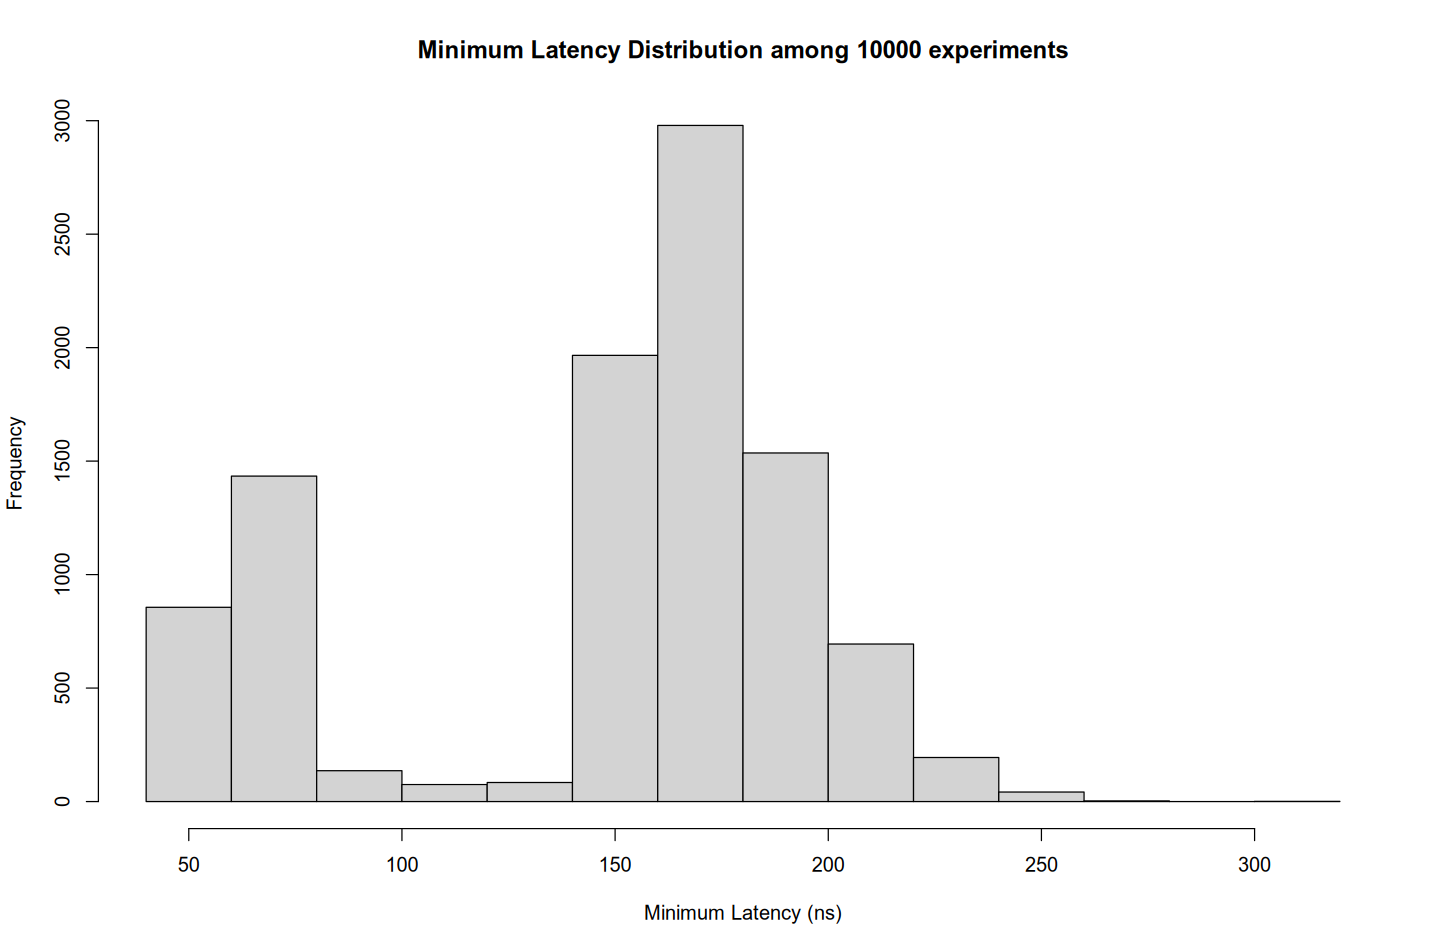
\includegraphics[width=0.75\textwidth]{./img/spinlock_first_try}
	\caption{Verteilung der Minima im ersten Experiment}
	\label{img:spinlock_first}
\end{figure}

Wie man sieht liegt, anders als zu erwarten wäre, keine Normalverteilung der Latenzen vor.
Nach reiflicher Überlegung hatte ich den Verdacht, dass ich durch die Instantiierung einer \texttt{Experiment}- und \texttt{Reader}-Objekts bei jedem Versuch eine große Menge ungenutzter Objekte erzeuge und dadurch ggf. der \emph{Garbage Collector} die Performance zeitweise mindert.

Um einen weiteren Performance-Faktor zu optimieren, habe ich noch die Konstruktion bestehend aus Boolean und synchronized Getter- und Settermethoden gegen einen \emph{AtomicBoolean} ausgetauscht.

Beim Herumexperimentieren wurde mir nun mit der Zeit klar, dass die Latenz derart gering sein muss, dass sie in der gleichen Größenordnung wie die Latenz der Zeitmessung selbst liegt.
Nachdem ich den Zeitmessungsprozess so weit ich konnte optimiert habe, sah der Prozess wie folgt aus:
\begin{lstlisting}[language=java,caption={Spinlocks: Latenzmessung im Main Thread (optimiert)}]
private void measure(int recursions) {
	long sendTime;
	long receiveTime;
	for (int i = 0; i < recursions; i++) {
		sendTime = System.nanoTime();
		lock.set(true);
		while (lock.get()) {
			// Do nothing (spinlock)
		}
		receiveTime = System.nanoTime();
		
		sendTimes.add(sendTime);
		receiveTimes.add(receiveTime);
	}
}
\end{lstlisting}

\begin{lstlisting}[language=java,caption={Spinlocks: Reader Thread (optimiert)}]
while (!isInterrupted()) {
	while (!experiment.lock.get()) {
		// do nothing (spinlock)
	}
	
	// Reset the lock (main thread is waiting)
	experiment.lock.set(false);
}
\end{lstlisting}

So wird jeweils die Zeit für einen Turn-Around gemessen, also die Zeit, die die Information von Main-Thread zum Reader-Thread und wieder zurück braucht.
Zum Berechnen der Latenz wird diese Zahl später durch zwei geteilt.
Allerdings ist hier immer noch auch die Latenz für das Abfragen und Speichern der aktuellen Zeit enthalten, was das Ergebnis in einer solch niedrigen Größenordnung durchaus verfälschen kann.

\subsection{Ergebnis}
Schlussendlich habe ich mich mit dem Versuch so zufrieden gegeben.
Ich habe 10000 Durchläufe des Experiments mit jeweils 50000 Rekursionen durchgeführt und jeweils die Minimalwerte der einzelnen Experimente zusammengetragen.
Von 10000 Durchläufen betrug die minimale Latenz 9854 mal \textbf{genau 64 Nanosekunden}.
Das spricht dafür, dass wir hier bereits an die Grenzen der Messgenauigkeit stoßen und daher ist die Berechnung eines Konfidenzintervalls eigentlich hinfällig. Hier aber trotzdem die geforderten Werte, auch wenn \textbf{ihre Aussagekraft durchaus angezweifelt werden kann}:
\begin{itemize}
	\item Durchschnittliche Minimallatenz: $63,95 ns$
	\item Untere Schranke des 95\%-Konfidenzintervalls: $63,92 ns$
	\item Obere Schranke des 95\%-Konfidenzintervalls: $63,98 ns$
\end{itemize}

Hier noch eine Wertetabelle, die alle gemessenen Minimallatenzen aufzeigt.

\begin{table}[H]
	\centering
	\label{tab:latencies}
	\begin{tabular}{|r|r|}
		\hline
		Latenz ($ns$) & Häufigkeit \\
		\hline
		24 & 7 \\
		30 & 1 \\
		35 & 1 \\
		40 & 12 \\
		64 & 9854 \\
		65 & 124 \\
		120 & 1 \\
		\hline
	\end{tabular}
\end{table}

\section{Aufgabe 2 - Latenz bei Kommunikation durch Semaphore}
\subsection{Versuchsaufbau / Implementierung}

Da ich nun schon sehr viel Zeit mit der Optimierung der Messung in Aufgabe 1 verbracht habe, habe ich mich entschieden, die Lösung zur besseren Vergleichbarkeit nur leicht abzuwandeln und Semaphoren anstelle des \texttt{AtomicBoolean} und \texttt{while}-Schleifen zu verwenden.
Der Ansatz zur Zeitmessung bleibt hier der gleiche: 
Es gibt zwei Semaphoren, eine \texttt{messageSemaphore} und eine \texttt{replySemaphore}, die beide zunächst blockiert sind.
Der Reader-Thread versucht, sobald er läuft, den Lock auf der \texttt{messageSemaphore} zu bekommen und gibt, wenn er den Lock bekommen hat, die \texttt{replySemaphore} frei.
Die Zeitmessung läuft im Main-Thread nun wiefolgt ab:
\begin{enumerate}
	\item Beginn der Zeitmessung
	\item \texttt{messageSemaphore} freigeben
	\item Versuche, Lock auf \texttt{replySemaphore} zu erhalten (warte auf Reader-Thread)
	\item Wenn der Lock erfolgreich erhalten wurde, stoppe die Zeitmessung
\end{enumerate}

Hier ein Auszug der entsprechenden Stellen aus dem Code:

\begin{lstlisting}[language=java,caption={Semaphores: Latenzmessung im Main Thread}]
private void measure(int recursions) {
	long sendTime;
	long receiveTime;
	for (int i = 0; i < recursions; i++) {
		sendTime = System.nanoTime();
		messageSemaphore.release();
		replySemaphore.acquire();
		receiveTime = System.nanoTime();
		
		sendTimes.add(sendTime);
		receiveTimes.add(receiveTime);
	}
}
\end{lstlisting}

\begin{lstlisting}[language=java,caption={Freigeben der replySemaphore im Reader Thread}]
while (!isInterrupted()) {
	try {
		experiment.messageSemaphore.acquire();
		experiment.replySemaphore.release();
	} catch (InterruptedException e) {
		System.out.println("Reader Thread shutting down.");
		break;
	}
}
\end{lstlisting}

So wird am ende durch Halbierung der gemessenen Zeit die durchschnittliche Latenz der beiden Wege berechnet und schließlich nach einer gegebenen Anzahl von Wiederholungen das Minimum abgespeichert.

\subsection{Ergebnis}
Bereits beim Testen ist mir anhand der Laufzeit aufgefallen, dass die Latenz bedeutend höher sein muss als in Aufgabe 1.
Um die Laufzeit gering zu halten, habe ich daher in dieser Versuchsreihe die Anzahl der Rekursionen auf 10000 reduziert und wie in Aufgabe 1 10000 Wiederholungen des Experiments durchgeführt.
Hier die Verteilung der Minimalen Latenzen über die 10000 Experimente:

\begin{figure}[H]
	\centering
	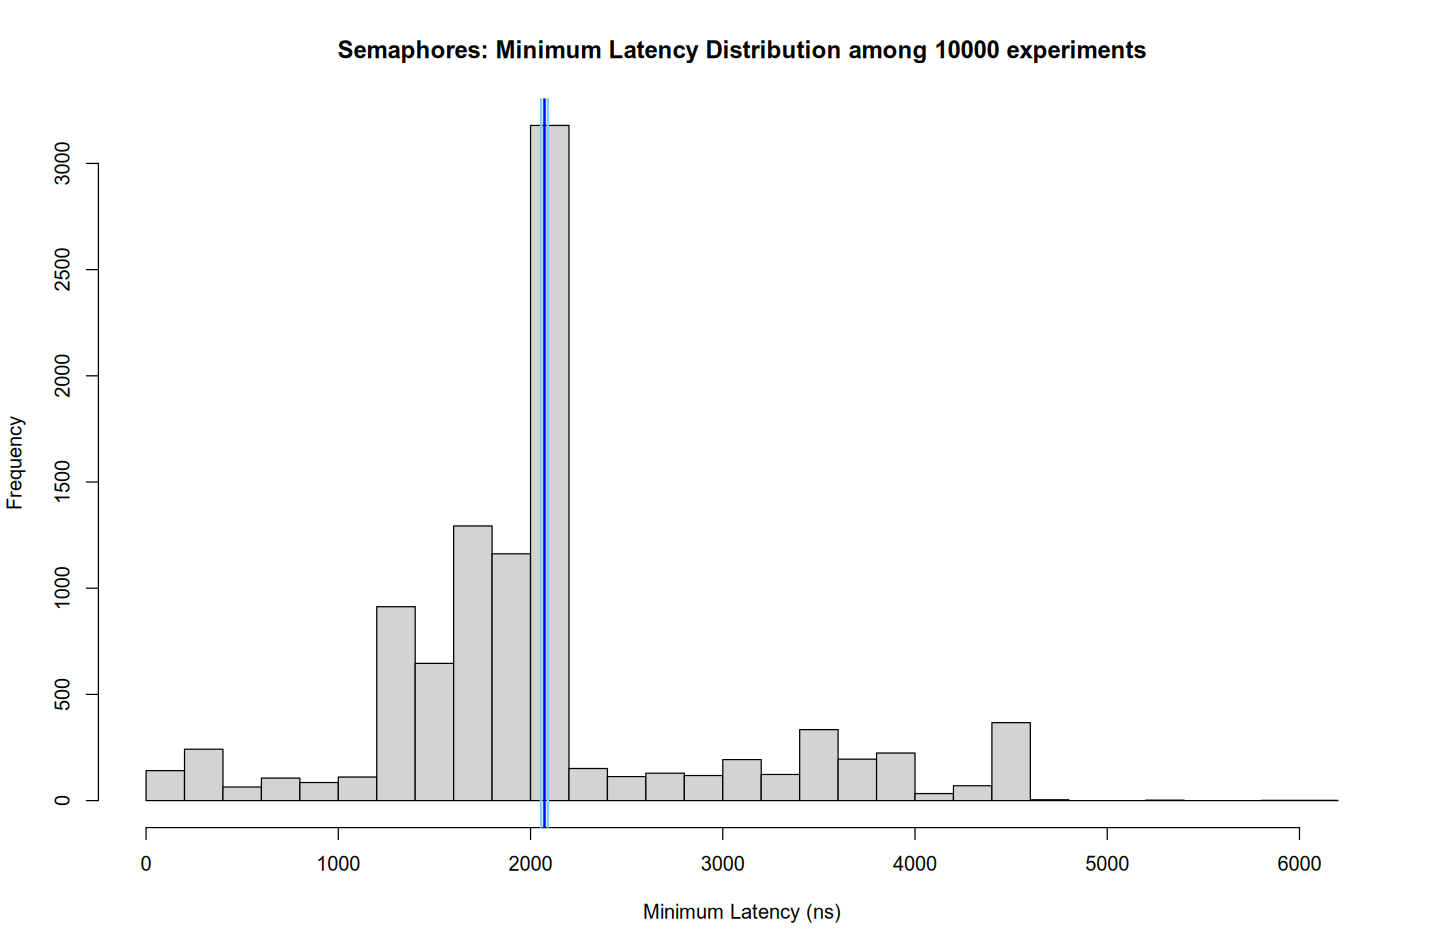
\includegraphics[width=0.75\textwidth]{./img/semaphores}
	\caption{Verteilung der Minima in der Versuchsreihe zu Aufgabe 2}
	\label{img:semaphore}
\end{figure}

Auch wenn sich hier eine Linksschiefe der Verteilung bemerkbar macht, gehe ich bei der Berechnung des Konfidenzintervalls (in Blau dargestellt) von einer Normalverteilung aus.
Der Grund für die Linksschiefe des Ergebnisses ist mir nicht ersichtlich.
Hier die Daten des 95\%-Konfidenzintervalls:
\begin{itemize}
	\item Durchschnittliche Minimallatenz: $2073 ns$
	\item Untere Schranke des 95\%-Konfidenzintervalls: $2055 ns$
	\item Obere Schranke des 95\%-Konfidenzintervalls: $2090 ns$
\end{itemize}

Die Latenz ist also um etwa zwei Zehnerpotenzen höher als bei der Verwendung von Spinlocks.
Dies ist auch nur logisch, da ein Thread in einem Spinlock alle ihm zur Verfügung stehenden Ressourcen verwendet, um zu überprüfen, ob der Lock freigegeben wurde.
Somit wird damit eine nahezu perfekte Latenz erzielt, jedoch bezahlt man den Preis dafür mit der CPU-Last, die ein Spinlock im Vergleich zu einer Semaphore hervorruft.
Wird ein Thread durch eine Semaphore blockiert, so wird er schlafen gelegt und verursacht nur eine sehr niedrige CPU-Last.

\section{Aufgabe 3 - Latenz bei Kommunikation mit ZeroMQ}
\subsection{Teil A (In-Process) - Versuchsaufbau / Implementierung}
Auch hier habe ich das Messungsverfahren aus den vorherigen Aufgaben nur leicht angepasst.
Anstelle der beiden Semaphoren kommen nun zwei PUSH-PULL Message Queues zum Einsatz: Eine befördert Nachrichten vom Main-Thread zum Reader-Thread, die andere in die entgegengesetzte Richtung.
Für den Socket wird als Protokoll \texttt{inproc} verwendet, welches die geringste Latenz bietet und für die Kommunikation innerhalb eines Prozesses gedacht ist.
Das grundsätzliche Vorgehen unterscheidet sich jedoch kaum:

\begin{lstlisting}[language=java,caption={ZeroMQ inproc: Latenzmessung im Main Thread}]
private void measure(int recursions) throws InterruptedException {
	long sendTime;
	long receiveTime;
	
	for (int i = 0; i < recursions; i++) {
		sendTime = System.nanoTime();
		sender.send(payload);
		receiver.recv();
		receiveTime = System.nanoTime();
		
		sendTimes.add(sendTime);
		receiveTimes.add(receiveTime);
	}
}
\end{lstlisting}

\begin{lstlisting}[language=java,caption={Antwort im Reader Thread}]
try {
	Socket receiver = context.createSocket(SocketType.PULL);
	receiver.connect("inproc://message");
	
	Socket sender = context.createSocket(SocketType.PUSH);
	sender.connect("inproc://response");
	
	while (!isInterrupted()) {
		receiver.recv();
		sender.send(payload);
	}
}
catch (Exception e) {
	System.out.println("Reader thread is shutting down");
}
\end{lstlisting}

Das Setup der ZeroMQ-Sockets im Main-Thread spare ich mir an dieser Stelle, das kann gerne im Code oder der Dokumentation nachgelesen werden.
Die \texttt{payload}, die hier als Nachricht und Antwort gesendet und empfangen wird, ist ein leeres Byte-Array, um unnötige Verzögerung durch die Nachrichtenübermittlung zu vermeiden und nur die Latenz zu messen.
Auch hier wird wieder die Zeit eines Round-Trips gemessen und dann halbiert, um die tatsächliche Latenz einer Nachrichtenübermittlung zu ermitteln.

\subsection{Teil A (In-Process) - Ergebnis}
Die gemessenene Minimallatenzen sind in der gleichen Größenordnung wie die in Aufgabe 2 gemessenen Latenzen, daher habe ich hier die gleichen Parameter gesetzt wie zuvor: 10000 Wiederholungen pro Experiment und insgesamt 10000 Durchläufe. Hier ein Histogramm der Verteilung:

\begin{figure}[H]
	\centering
	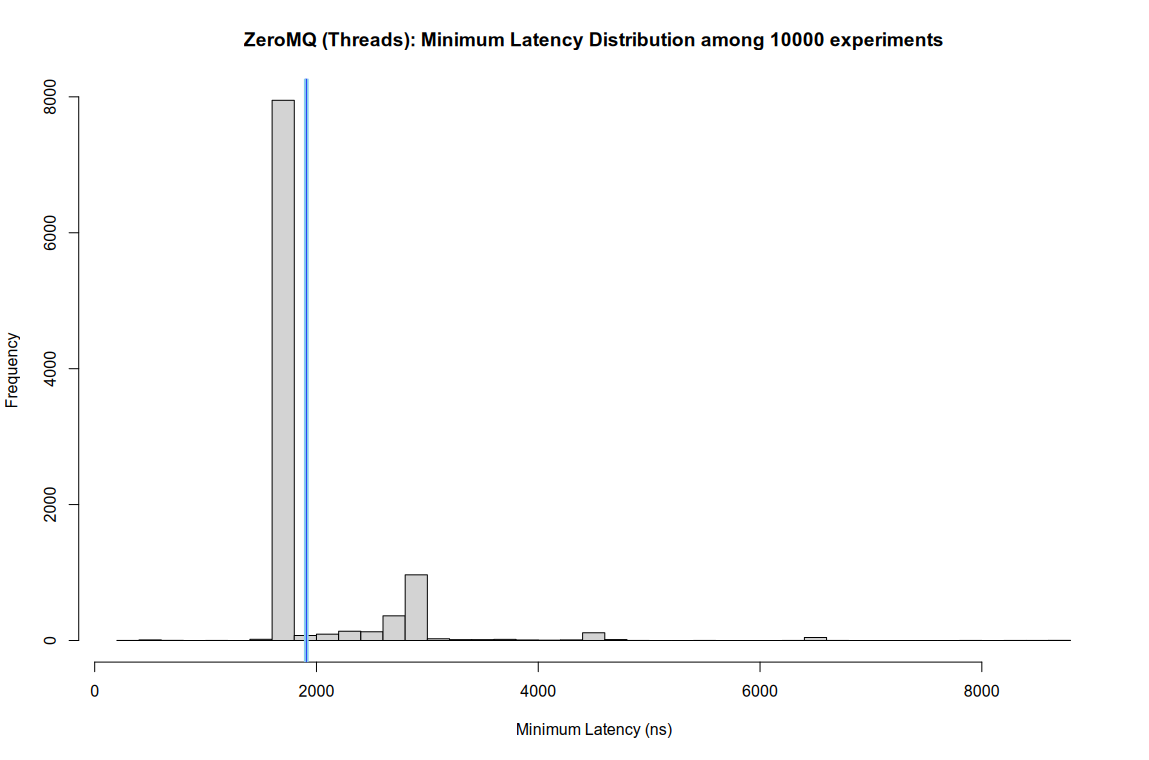
\includegraphics[width=0.75\textwidth]{./img/zeromq_inproc}
	\caption{Verteilung der Minima in der Versuchsreihe zu Aufgabe 3A}
	\label{img:zeromq:inproc}
\end{figure}

Das Konfidenzintervall ist hier wieder in Blau dargestellt.
Hier nochmal die genauen Werte:
\begin{itemize}
	\item Durchschnittliche Minimallatenz: $1908 ns$
	\item Untere Schranke des 95\%-Konfidenzintervalls: $1869 ns$
	\item Obere Schranke des 95\%-Konfidenzintervalls: $1921 ns$
\end{itemize}

Wie man sieht, unterbietet ZeroMQ hier die Latenz der Semaphore leicht, was ich durchaus bemerkenswert finde.

\subsection{Teil B (Inter-Process) - Versuchsaufbau / Implementierung}
Nachdem ZeroMQ schon mal eingebaut war, war der Schritt von In-Process- zu Inter-Process-Kommunikation nicht mehr weit:
Ich musste bloß den Worker Thread in ein eigenes Programm umwandeln (Code aus run()-Methode des Threads in eine eigene main-Methode verschieben) und einen eigenen ZeroMQ-Kontext darin verwalten.
Zusätzlich wird nun als Protokoll nicht mehr \texttt{inproc}, sondern \texttt{ipc} verwendet, welches über \emph{UNIX domain sockets} kommuniziert.

\begin{lstlisting}[language=java,caption={Antwort im Reader Thread}]
public static void main(String[] args) {
	try(ZContext context = new ZContext()) {
		Socket receiver = context.createSocket(SocketType.PULL);
		receiver.bind("ipc:///tmp/zmq-message.sock");
		
		Socket sender = context.createSocket(SocketType.PUSH);
		sender.bind("ipc:///tmp/zmq-response.sock");
		
		System.out.println("Listening now");
		while (true) {
			receiver.recv();
			sender.send(payload);
		}
	}
	catch (Exception e) {
		System.out.println("Reader is shutting down");
	}
}
\end{lstlisting}


Im Main-Programm musste dafür nur der Connect-String entsprechend angepasst werden bei der Erstellung der Socket-Objekte.

\subsection{Teil B (Inter-Process) - Ergebnis}
Da die Ergebnisse und somit die Laufzeit nun eine weitere Zehnerpotenz größer wurden, habe ich zum Ausgleich die Anzahl der Versuchsdurchläufe auf 1000 reduziert. Dadurch leidet die Präzision des errechneten Konfidenzintervalls, der Unterschied im Vergleich zu den vorhergegangenen Aufgaben ist aber dennoch offensichtlich.
Hier ein Histogramm der Messwerte:

\begin{figure}[H]
	\centering
	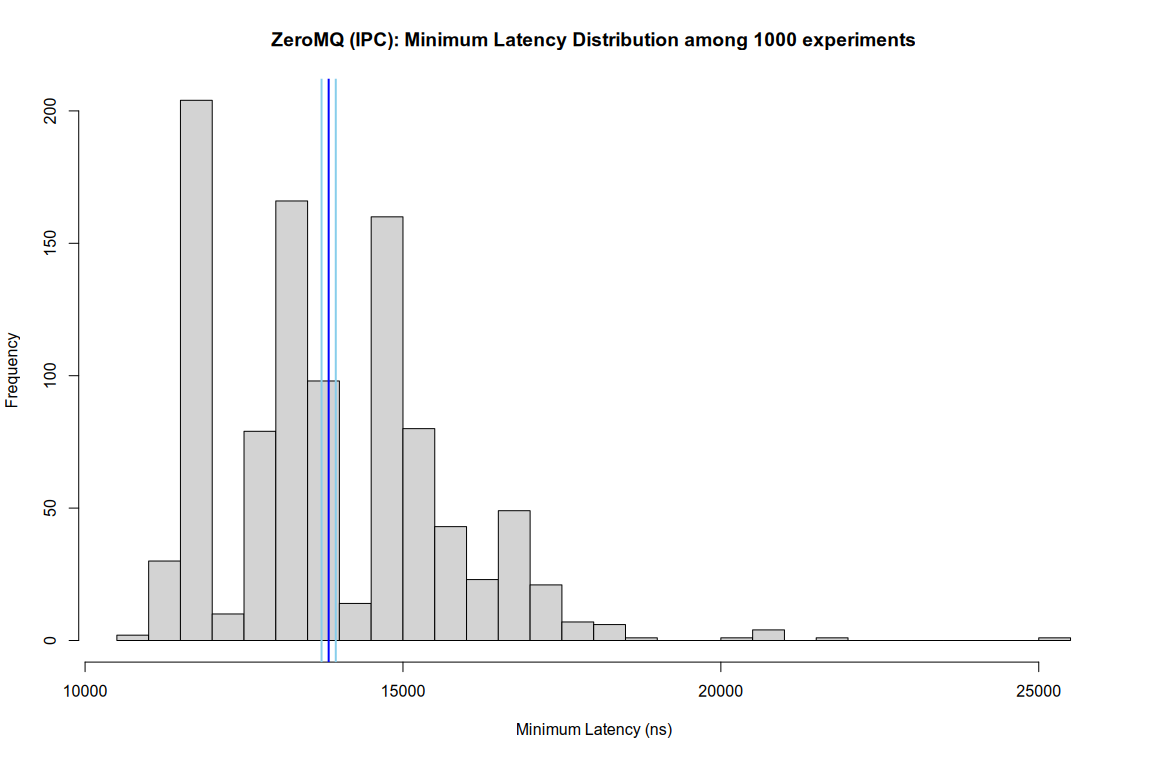
\includegraphics[width=0.75\textwidth]{./img/zeromq_ipc}
	\caption{Verteilung der Minima in der Versuchsreihe zu Aufgabe 3B}
	\label{img:zeromq:ipc}
\end{figure}

Auch hier ist nur mit etwas Phantasie eine Normalverteilung zu erkennen, da die Ergebnisse recht lückenhaft sind.
Trotzdem gehe ich hier wieder von einer Normalverteilung aus und berechne entsprechend das in Blau dargestellte 95\%-Konfidenzintervall:

\begin{itemize}
	\item Durchschnittliche Minimallatenz: $13,83 \mu s$
	\item Untere Schranke des 95\%-Konfidenzintervalls: $13,72 \mu s$
	\item Obere Schranke des 95\%-Konfidenzintervalls: $13,94 \mu s$
\end{itemize}

\section{Aufgabe 4 - Kommunikation zwischen Docker-Containern}
\subsection{Versuchsaufbau / Implementierung}
Auch hier konnte ich wieder auf die Vorarbeit aus den vorherigen Aufgaben zurückgreifen:
Da ZeroMQ auch die Kommunikation über TCP unterstützt, ist es sehr gut geeignet, um auch über ein Docker-Netzwerk zwischen Docker-Containern zu kommunizieren.
Diesmal mussten dafür ausschließlich die Socket-Bezeichnungen im Java-Code aus Aufgabe 3B angepasst werden und der Dateiname der Output-Datei.
Zusätzlich dazu habe ich je ein Dockerfile für den Reader und den Writer erstellt und schließlich das ganze Projekt mit Netzwerk-Setup und Volume-Einbindung in einem \texttt{compose.yaml} zusammengefasst.

\subsection{Ergebnis}
Die Ergebnisse liegen in einer ähnlichen Größenordnung wie jene aus Aufgabe 3B, daher war keine weitere Verringerung der Wiederholungen notwendig.
Hier die Ergebnisse:
\begin{figure}[H]
	\centering
	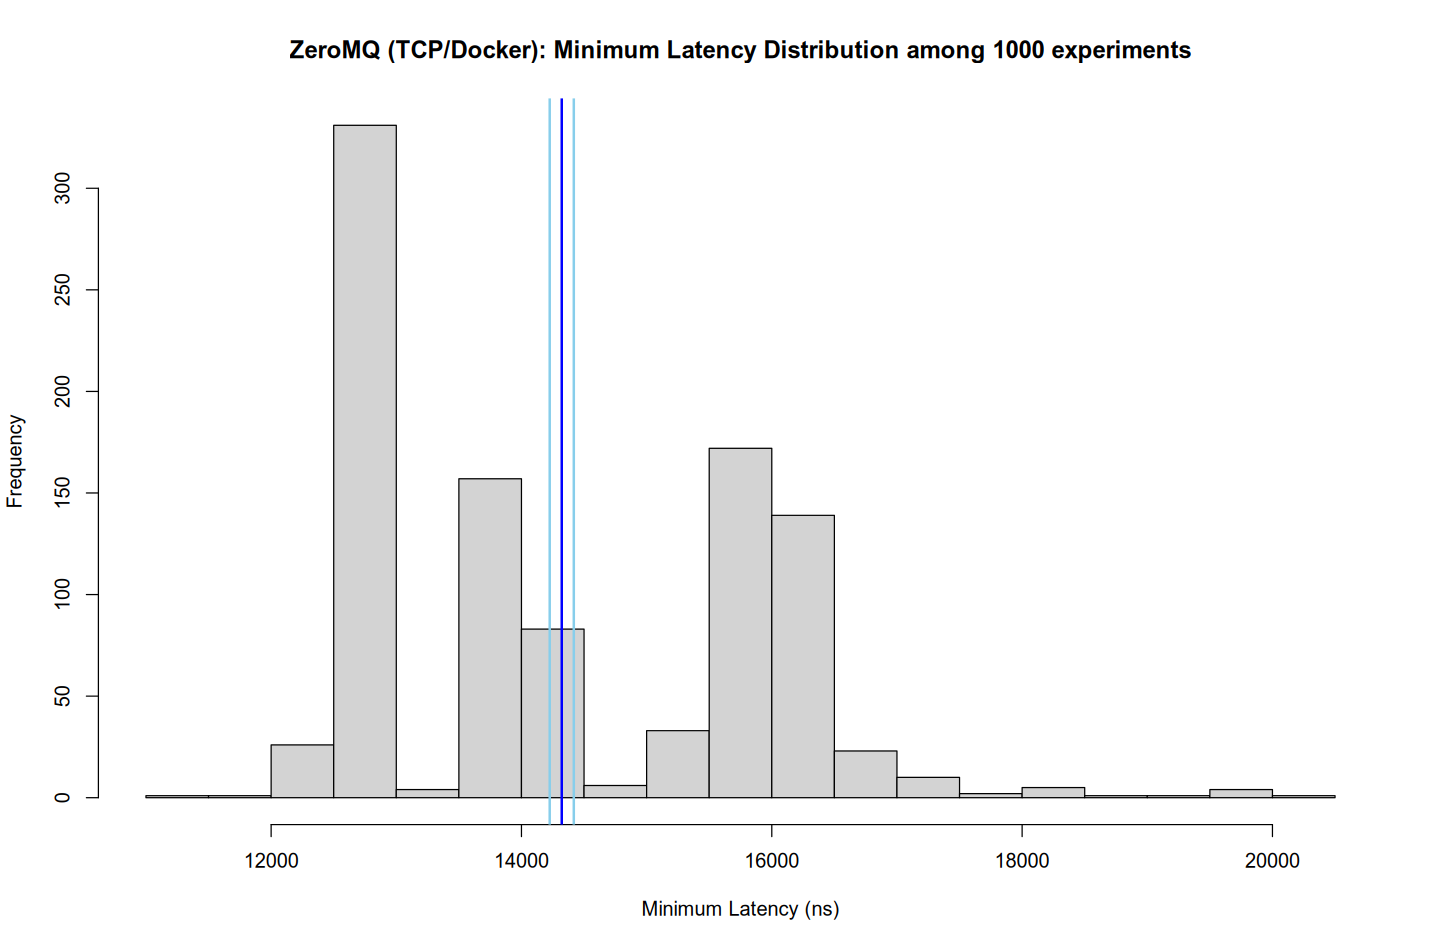
\includegraphics[width=0.75\textwidth]{./img/zeromq_docker}
	\caption{Verteilung der Minima in der Versuchsreihe zu Aufgabe 4}
	\label{img:zeromq:docker}
\end{figure}

Auch hier liegt nicht wirklich eine Normalverteilung vor, trotzdem hier nochmal die Eckdaten des in Blau eingezeichneten Konfidenzintervalls:

\begin{itemize}
	\item Durchschnittliche Minimallatenz: $14,32 \mu s$
	\item Untere Schranke des 95\%-Konfidenzintervalls: $14,23 \mu s$
	\item Obere Schranke des 95\%-Konfidenzintervalls: $14,42 \mu s$
\end{itemize}

Somit liegt die minimale Latenz im Durchschnitt etwas höher als die Latenz bei IPC-Kommunikation. 
Der Overhead durch Docker scheint also sehr gering zu sein, da die Verwendung von TCP an sich bereits einen Overhead mit sich bringt.

\section{Abschließende Gedanken}
Wie zu erwarten war, ist die Latenz bei Nutzung eines Spinlocks am geringsten, da hier nur wenige Maschineninstruktionen im Prozess involviert sind.
Verwendet man Semaphoren, so nimmt die Latenz bereits deutlich zu, jedoch wird dadurch der Overhead an verschwendeter Rechenleistung vermieden, den ein Spinlock erzeugt.
Erstaunlich finde ich, dass die Kommunikation über ZeroMQ sogar eine etwas geringere Latenz aufweist als die Kommunikation per Semaphore, da die Semaphore ja bereits ein Feature auf Betriebssystem-Basis ist.
Ad-Hoc kann ich mir diesen Vorteil auch nicht erklären.

Je weiter man nun die Distanz von Empfänger und Sender erhöht, desto mehr steigt auch die Latenz - so weit, so erwartbar.
Hier ist allerdings interessant zu sehen, wie wenig Unterschied es macht, ob Sender und Empfänger nur in verschiedenen Prozessen laufen und über UNIX domain sockets kommunizieren, oder ob sie in verschiedenen Docker-Containern laufen und per TCP miteinander kommunizieren.

Ein Punkt, den ich noch ansprechen möchte, ist die Verteilung der Ergebnisse. 
Oftmals lässt sich in den Ergebnissen, anders als meiner Ansicht nach zu erwarten wäre, keine Normalverteilung erkennen. 
Stattdessen sieht man schiefe Verteilungen und sogar Verteilungen mit mehreren lokalen Maxima.
Um mir die Sache nochmal besser zu veranschaulichen, habe ich Scatterplots der Versuchsreihen erstellt, in denen diese Tendenz nochmal besser sichtbar wird:

\begin{figure}[H]
	\centering
	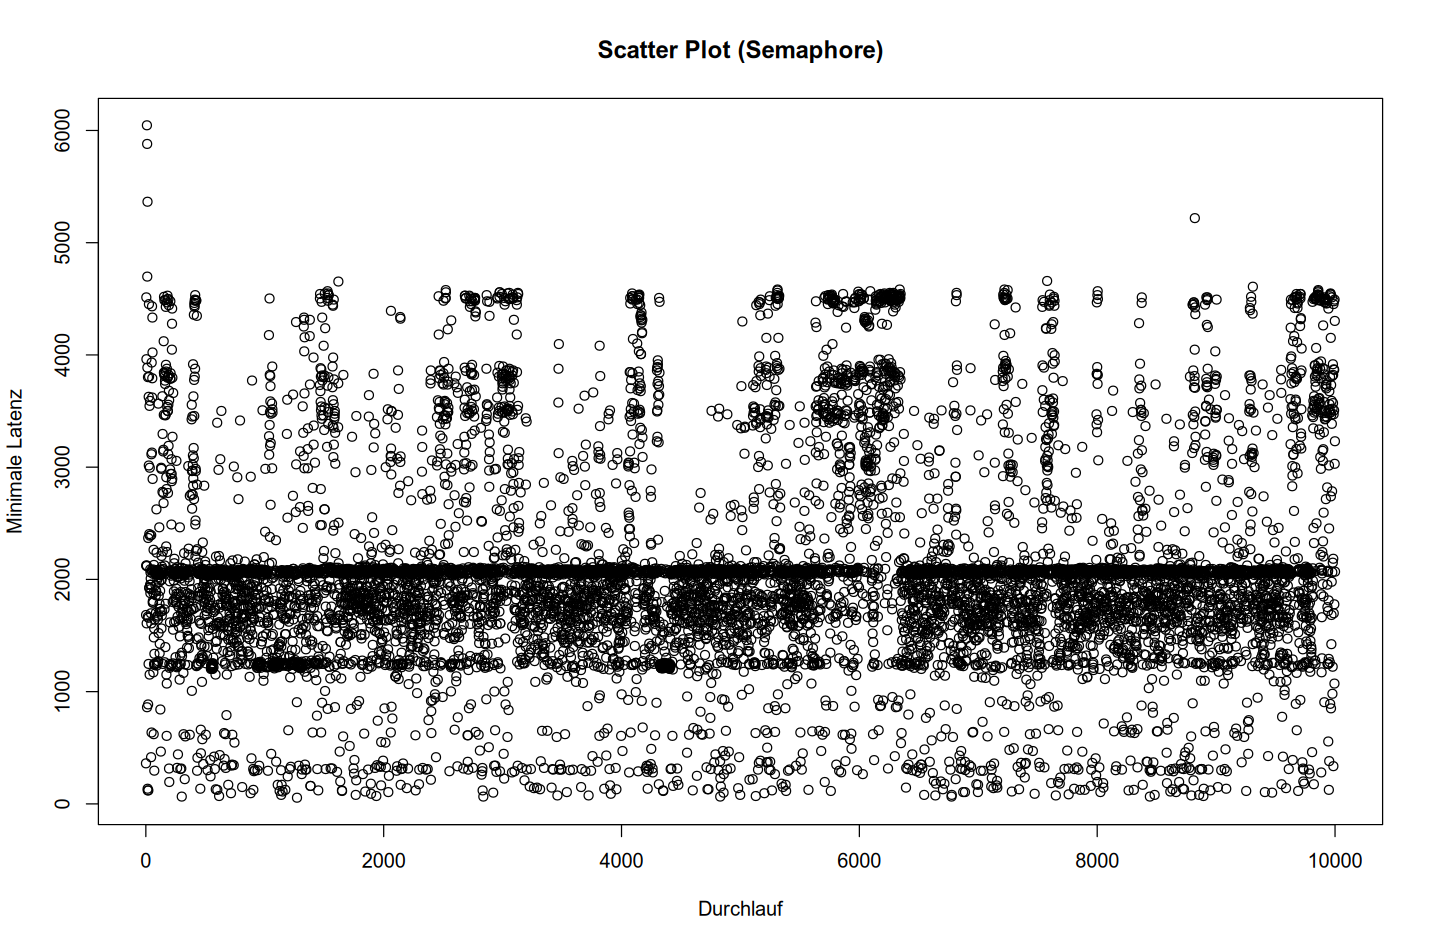
\includegraphics[width=0.75\textwidth]{./img/scatter_semaphore}
\end{figure}
\begin{figure}[H]
	\centering
	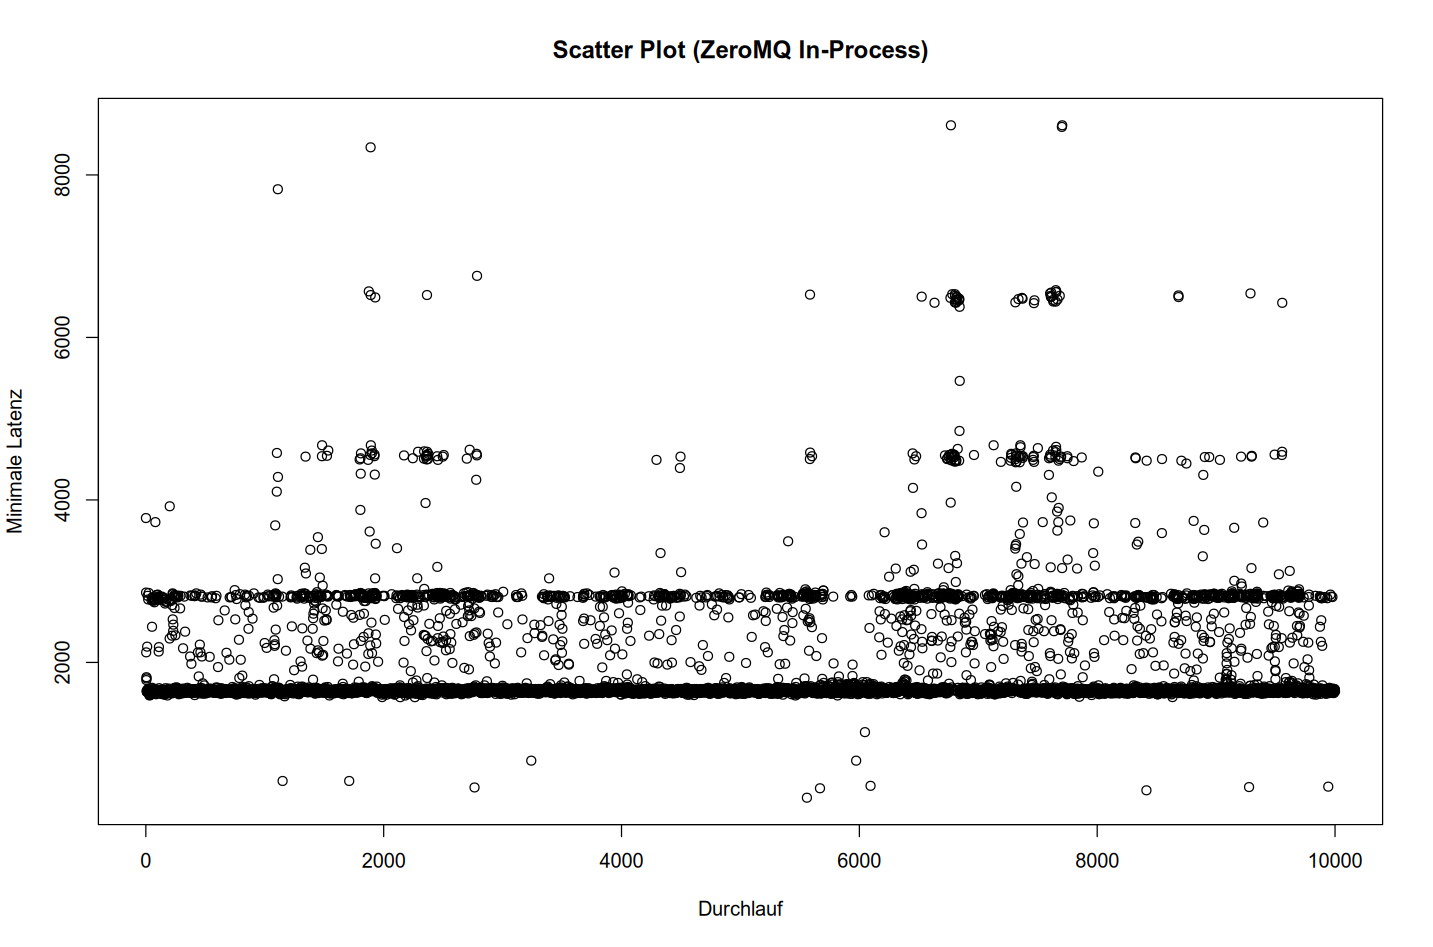
\includegraphics[width=0.75\textwidth]{./img/scatter_inproc}
\end{figure}
\begin{figure}[H]
	\centering
	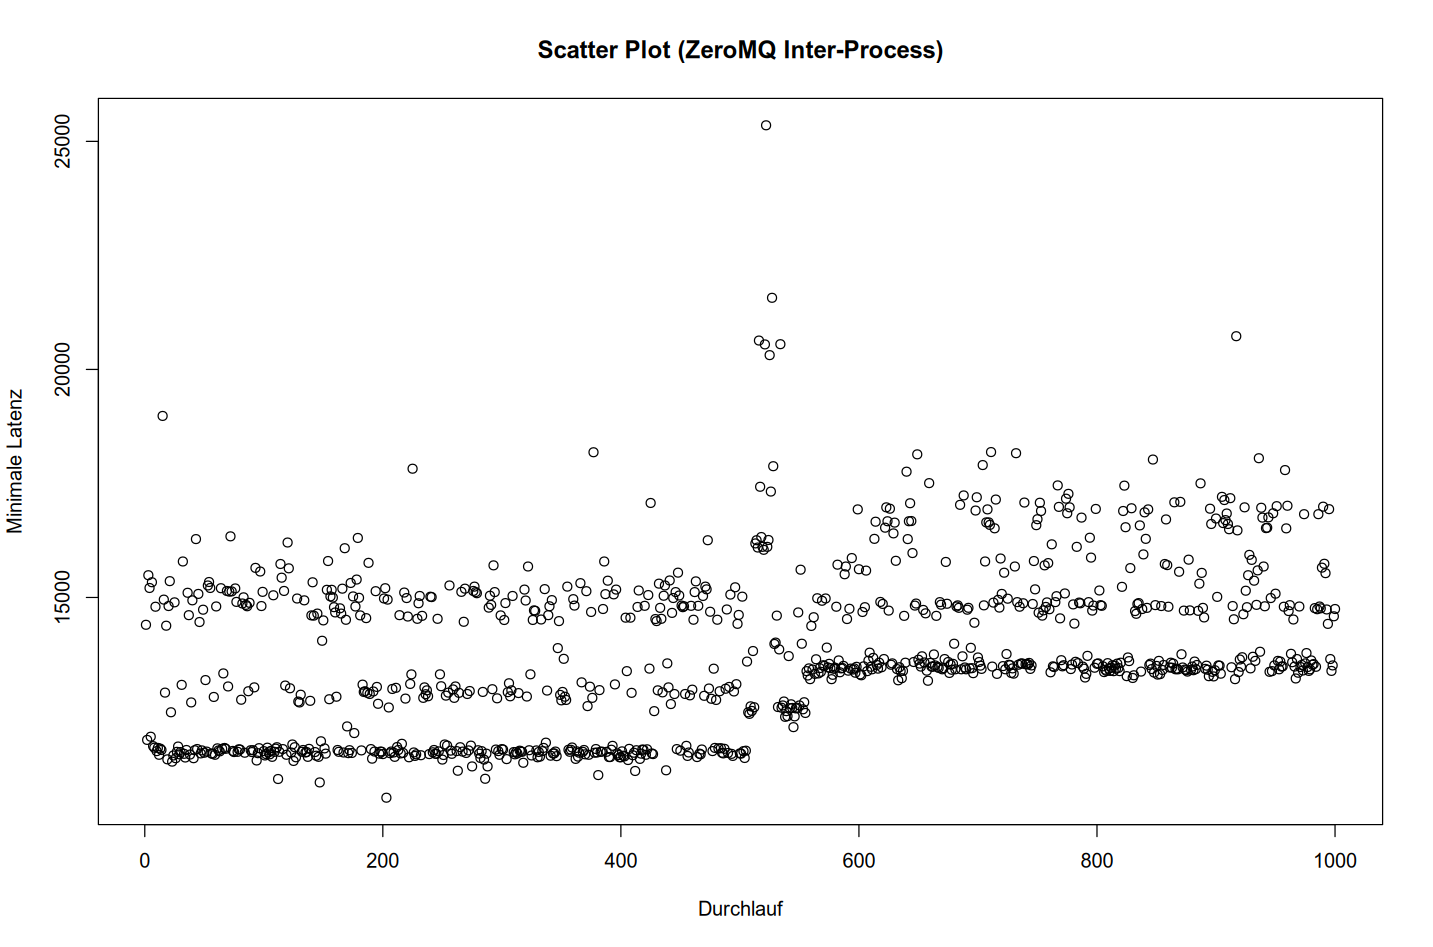
\includegraphics[width=0.75\textwidth]{./img/scatter_ipc}
\end{figure}
\begin{figure}[H]
	\centering
	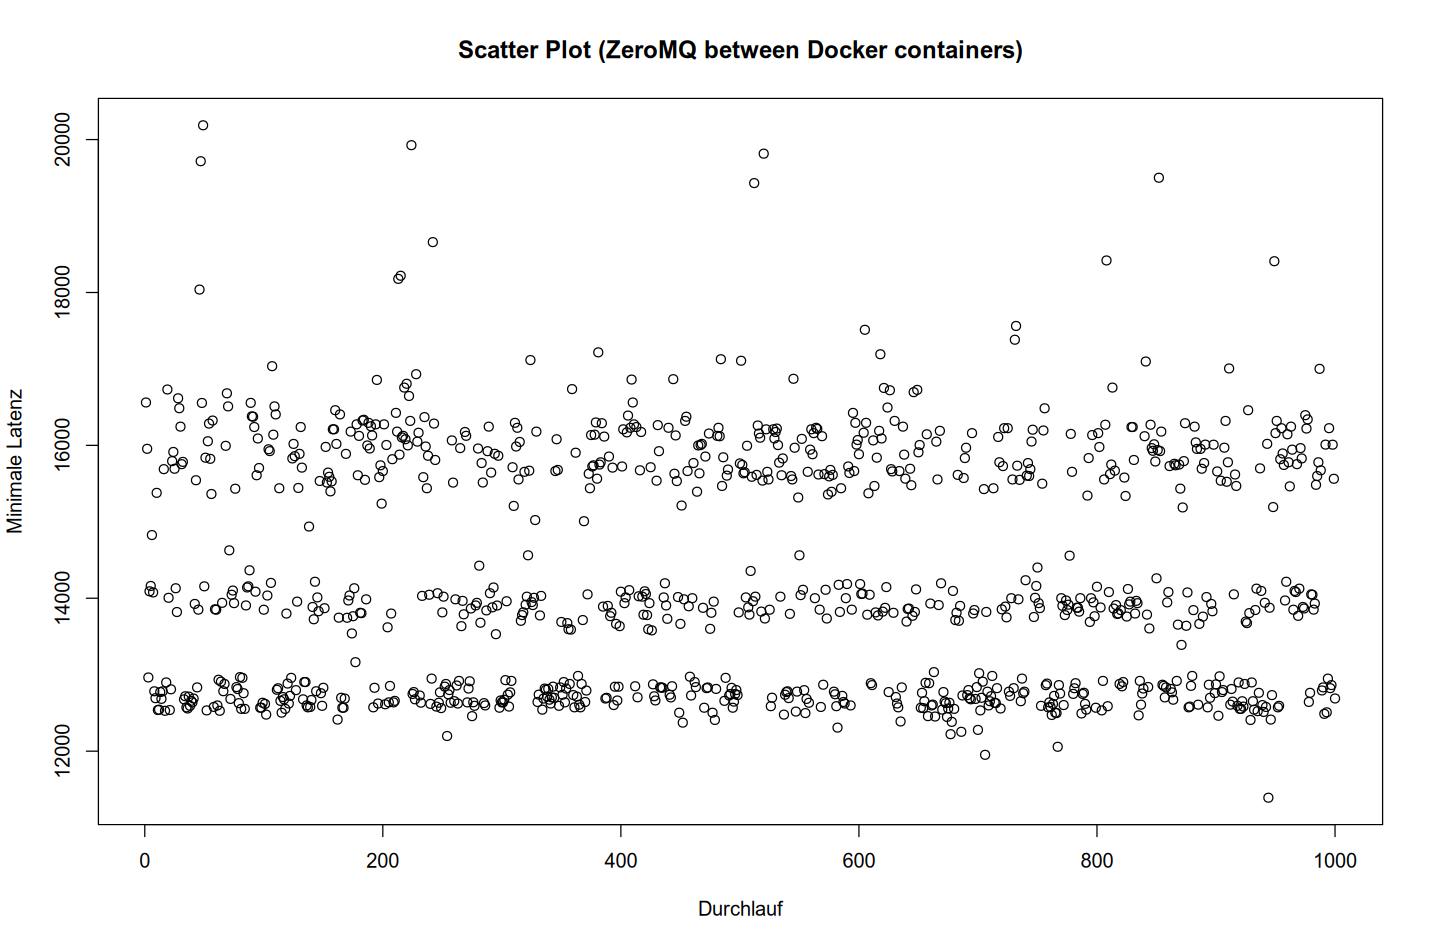
\includegraphics[width=0.75\textwidth]{./img/scatter_docker}
\end{figure}

Besonders bei den Versuchen mit Semaphoren und ZeroMQ mit In-Process-Kommunikation sind hier die Linien sehr deutlich zu sehen, aber auch in den anderen beiden Versuchen wird eine solche Tendenz sichtbar.

Meine Theorie dazu ist, dass auch bei Semaphoren und ZeroMQ eine Art von Polling verwendet wird, um festzustellen, ob die Semaphore nun frei geworden ist bzw. ob eine Nachricht in der Queue anliegt.
Wenn also zum Zeitpunkt $t_1$ gepollt wird und keine Nachricht anliegt, so vergeht mindestens eine konstante Zeit $\Delta t$ bis erneut gepollt wird und eine Chance besteht, dass die Nachricht gelesen wird, selbst wenn sie eigentlich schon sofort nach dem Verstreichen von $t_1$ gelesen werden könnte.

Auch fällt ins Auge, dass bei der IPC-Variante (Aufgabe 3B) nach der Hälfte der Versuche die minimalen Latenzen für den Rest der Versuchsreihe stark ansteigen.
Dieses Phänomen ist bei mehreren Versuchen immer wieder aufgetreten und mir fällt keine vernünftige Erklärung dafür ein.

\section{Anleitung zum Selber-Testen}
Damit die Tests auch von motivierten Leser*innen nachgestellt werden können, habe ich in den entsprechenden Ordnern README-Dateien mit Instruktionen platziert.

Die R-Skripte, die für die Auswertung verwendet wurden, liegen im Ordner \texttt{statistics}. Dort muss vor der Verwendung das Arbeitsverzeichnis (je erster Befehl) geändert werden auf den tatsächlichen Ort des \texttt{statistics}-Ordners.
Oder R direkt dort ausführen, das sollte auch gehen.
Ich empfehle RStudio, um die Befehle Schritt für Schritt auszuführen und die Zwischenergebnisse zu sehen.

\end{document}